\documentclass{article}
\usepackage[utf8]{inputenc}
\usepackage[danish]{babel}
\usepackage{palatino}
\usepackage{float}
\usepackage{url}
\usepackage{graphicx}
\newcommand{\env}[1]{\textit{#1}}
\newcommand{\fname}[1]{\textbf{\texttt{#1}}}
\newcommand{\cmd}[1]{\textbackslash \texttt{#1}}
\newcommand{\shellcmd}[1]{\texttt{#1}}
\newcommand{\envbegin}[1]{\cmd{begin}\{\env{#1}\}}
\newcommand{\envend}[1]{\cmd{end}\{\env{#1}\}}
\newcommand{\term}[1]{\textbf{\textit{#1}}}
\newcommand{\example}[1]{``\texttt{#1}''}
\linespread{1.05}
\title{Vejledning i brug af RevyTEX\\Version 0.9.2}
\author{Ronni Elken Lindsgaard}

\begin{document}
\maketitle
Denne vejledning er en guide i hvordan man skriver sketches og sange i
tex-format samtidig hvordan man bygger manuskripter m.v. efterfølgende.
\section{Disclaimer}
Dette dokument er skrevet for at lette arbejdet med RevyTeX kataloget
for de forskellige revy på natfak. Det forudsættes ikke at man ved
hvordan man skal skrive TeX-kode, men følger man vejledningen
minutiøst bør det ikke være et problem. Latex kan overættes på alle
former for styresystemer, men RevyTeX er skabt til at køre på Linux.
Jeg vil i sektionen om RevyTeX antage at man bruger Ubuntu. Hvis du
kører en anden distribution er du nok i stand til at vide hvad du skal
gøre alligevel.

Guiden er forfattet af Ronni Elken Lindsgaard og bygger på mine egne
erfaringer med brug af \fname{revy.sty} filen og RevyTex-kataloget og
skal ikke ses som en udtømmende vejledning i at bruge noget af det.
Skabelonerne er forfattet af Bjarke Mønsted i forbindelse med FysikRevy.
Jeg håber det kan bruges. Har man rettelser til fejl eller spørgsmål til
vage formuleringer bedes man maile
\texttt{ronni@diku.dk} så vil jeg forsøge at rette dem efter bedste
evne. Vejledningen har hjemme på \url{github.com/dikurevy/vejledning} og
tjek venligst denne version om de fejl du har fundet er rettet.

\subsection{Licens}
Dokumentet og skabelonerne er frigivet under en 'Beerware' licens der
lyder som følger:

Brug og distribuér dokumentet og skabelon-filer som du har lyst til. Men
lad være med at tage penge for det, og hold informationen om forfattere
intakt. Forfatterne kan
på ingen måde holdes ansvarlig for hvad du bruger det til og eventuelle
skader de forsåger på din eller andres computere (men held og lykke med
at overtage verdensherredømmet!). Hvis du
møder os og synes det vi har lavet er 1337 så er du mere end velkommen
til at honorere os med en øl eller hvad vores smagsløg lige står og
begærer.

\section{At skrive sketches og sange}
Placer \fname{revy.sty} filen i den mappe hvor du vil gemme dine
sketches og sange. I din tex-fil skal du bruge '\cmd{usepackage}\{revy\}' som
så vil inkludere \fname{revy.sty}. Hvis du har lyst kan du også installere
sty-filen i dine tex-pakker, i så fald ved du nok selv hvordan man gør.

\subsection{Tex-filens opbygning}
Her er en beskrivelse af de forskellige kommandoer revy.sty stiller til
rådighed. Hvis du bruger skabelon.tex som udgangspunkt er der flere af
disse kommandoer du nok ikke behøver vide hvad gør.
Syntaksen er som følger. Argumenter angives enten i tuborg-klammer eller
kantede parenteser - den følgende beskrivelse beskriver præcis hvornår
hvad skal bruges. Såkaldte \term{environments} skabes ved at skrive
'\envbegin{environment}' og sluttes ved at skrive
'\envend{environment}'.
Som udgangspunkt er det en god idé at kopiere \fname{skabelon.tex} og rette til
derefter.

\begin{description}
\item[\cmd{revyname} \{\}:] Revyens navn e.g "DIKUrevy"
\item[\cmd{revyyear}\{\}:] Året hvor revyen afspilles e.g. "2012"
\item[\cmd{version}\{\}:] Hvilken version sketchen/sangen er i.
\item[\cmd{eta}\{\}:] Hvor lang tid sketchen forventes at tage.
\item[\cmd{status}\{\}:] Status for sketchen.
\item[\cmd{title}\{\}:] Sketchen/sangens titel som den fremgår af aktoversigt mv.
\item[\cmd{author}\{\}:] Forfatter(e) af sketchen/sangen.
\item[\envbegin{roles} .. \envend{roles}:]
Definition af \env{roles}-environmentet.
Indsættes efter \envbegin{document} men før \envbegin{sketch} eller
\envbegin{song}. Bruges til at definere hvilke roller der er i en
sketch/sang.
\item[\cmd{role}\{ \} {[]}:] Indsættes i \env{roles}-environmentet. Første argument (i
tuborg-klammer) bruges
til at angive forkortelsen af rollen og bruges videre i tex-filen. Andet
argument (i kantede parenteser) er skuespilleren der har fået rollen (dette bliver brugt af
andre scripts, så hver konsekvent med navngivning) og til sidst navn/beskrivelse på
rollen. Indsæt ny \cmd{role} på en ny linje for læsbarhed.
\item[\envbegin{props} .. \envend{props}:] Definition af \env{props}-environment.
Indsættes på samme måde som \env{roles}-environmentet. Bruges til at
definere en liste af rekvisitter som bruges i sketchen som udskrives for
sig til rekvisitfolkene.
\item[\cmd{prop}\{\}{[]}:] Indsættes i \env{props}-environmentet. Første argument (i
tuborg-klammer) er navnet på rekvisitten f.eks. 'Oracle server'. Andet
argument (i kantede parenteser) er angivelse af en person som kan skaffe
denne rekvisit. Efterfølgende beskrives rekvisitten evt. nærmere med
størrelse eller andre detaljer såsom hvad den skal bruges til (det
hjælper rekvisitfolkene med at vide hvad de skal lave). e.g. 'Skal
bruges til at danse rundt om og 2 personer skal kunne gemme sig bag
den'.
\item[\envbegin{mics} .. \envend{mics}:] Definition af \env{mics}-environmentet.
Indsættes på samme måde som \env{roles}- og \env{props}-environmentsne. Bruges til at generere
en liste over hvem der bruger mikrofoner i hvilke sketches hvornår til
texnikken.
\item[\cmd{mic}\{\}:] Indsættes i \env{mics}-environmentet. Første argument (i
tuborg-klammer) angiver hvilket mikrofon der er tale om (HS1-HS4 og
MIC1-MIC4). Angiv samme navn på skuespiller som under \env{roles}.
\item[\cmd{scene}\{\}:] Angiver ting der sker på scenen. e.g.
\example{\cmd{scene}\{D1 viser D2 bogen\}}
bogen'. Denne kommando kan bruges både i \env{sketch}- og
\env{song}-environmentsne.
\item[\envbegin{sketch} .. \envend{sketch}:] Definition af \env{sketch}-environmentet. 
\item[\cmd{says}\{\}:] Argumentet (i tuborg-klammer) angiver hvem der siger
følgende. Brug samme forkortelser som i \env{roles}. Kan bruges i
\env{sketch}-environmentet
\item[\envbegin{song} .. \envend{song}:] Definition af \env{song}-environmentet.
\item[\cmd{sings}\{\}{[]}] Første argument (i tuborg klammer) angiver
hvilken del af sangen der synges e.g. 'vers1, omkv osv'. Andet argument
(i kanteder paranteser) angiver hvem der synger. Brug samme forkortelser
som i \env{roles}. Kommandoen kan kun bruges i \env{song}-environmentet.
\item[\cmd{act}\{\}:] Angiver noget rollen gør. Anvendes typisk i
forbindelse med \cmd{sings} eller \cmd{says}. e.g. \example{\cmd{says}\{D1\}
Hallooo bedste, \cmd{act}\{banker på døren\} luk mig ind lissom.}
\end{description}

\subsection{Tilføjelse til revykatalog}
Der er forskelligt hvordan revyerne giver adgang til revykataloget. Det
kan enten være vha. ftp, ssh eller en helt tredje mulighed. Her følger
kun en beskrivelse af mappestrukturen i RevyTeX-kataloget

\begin{description}
\item[\fname{kontakter/}] Denne mappe indeholder kontaktinformationer på alle i
revyen formateret til 'vcf'-formatet. En let måde at bygge denne
kontaktliste på er ved at indtaste kontaktinformationer i gmail og
derefter eksportere dem i 'vCard format'.
\item[\fname{sange/}] Heri lægges alle sange. Det er kun nødvendigt at lægge
selve tex-filerne i mappen da pdf'erne genereres automatisk.
\item[\fname{sketches/}] Heri lægges alle sketches. Det er kun nødvendigt at
lægge selve tex-filerne i mappend da pdf'erne genereres automatisk.
\item[\fname{video/}] Heri lægges videoer og pausefisk. Der findes endnu intet
miljø til videoer, men de skal defineres for at kunne fremgå i
aktoversigt m.m. Brug sketch-skabelonen til formålet.
\end{description}

\section{RevyTeX administration}
\subsection{Installation af RevyTeX}
%get moreverb package (texlive-latex-extra or
%http://ctan.org/tex-archive/macros/latex/contrib/moreverb)
%text-vcard hentes seperat
%perl -MCPAN -e 'install HTML::Template'
%YAML::Any
%JSON::XS
%Text::vCard
%File::Slurp
%File::Slurp::Unicode
%PDF::Reuse
%PDF::API2
%Makefile::Parser
\begin{enumerate}
\item Navigér til den mappe hvor RevyTeX skal bo. evt. \shellcmd{mkdir
revy \&\& cd revy}
\item Hent RevyTeX med \shellcmd{git clone
git://github.com/dikurevy/RevyTeX.git} eller hent zip-filen fra
\url{http://github.com/dikurevy/RevyTeX} (og læg RevyTex mappen i mappen
fra skridt 1.
\item I en terminal kør 
\begin{verbatim}
sudo apt-get install libjson-xs-perl \
libfile-slurp-unicode-perl \
libmakefile-parser-perl \
libtext-vcard-perl \
libpdf-reuse-perl \
libpdf-api2-perl
\end{verbatim} som vil installere alle
perl pakker der er nødvendige. (hvis \shellcmd{libfile-slurp-unicode-perl} ikke
er tilgængelig, forsøg blot med \shellcmd{libfil-slurp-perl} eller find modulet File::Slurp::Unicode på
\url{http://cpan.org} og installér)
\item Hent og installér \LaTeX-pakken \textit{moreverb} på
\url{http://ctan.org/pkg/moreverb} eller kør \shellcmd{sudo apt-get
install texlive-latex-extra} som vil installere en hel masse
\LaTeX-pakker (ca 350MB).
\item \$\$\$.
\end{enumerate}

\subsection{Oprettelse af RevyTeX-katalog}
Navigér til RevyTeX-mappen med en terminal. Indtast kommandoen \shellcmd{make
../20xx} hvor \texttt{20xx} er den mappe som kataloget vil blive gemt
som.\footnote{Bemærk at stien til den nye mappe skal være præfikset med \shellcmd{../}
dette gør at det nye katalog lægger sig i samme mappe som RevyTeX mappen
og ikke som en undermappe -- som foråsager at nogle af scriptsne ikke
kan finde ud af stien.}
Terminalen vil spørge om revyens navn og årstal. Når disse er indtastet
vil kataloget blive oprettet.

\subsection{Bygning af manuskripter og filer}
Når manuskripterne skal bygges oprettes først filen
\fname{aktoversigt.plan}
som indeholder en liste over alt materiale der er med i revyen. Formatet
er således:

Første linie og første linie efter en blank linie er akt-overskriften
f.eks. 'Akt 1', 'Akt 2' mv. Herefter følger listen af sange og sketches
i aktet i ordnet rækkefølge. Man lister stien til
sketchen/sangen/videoens tex-fil relativt fra roden af
RevyTeX-kataloget. f.eks. for sketchen \fname{minfoerstesketch.tex} som ligger
i sketches-mappen skrives linjen \fname{sketches/minfoerstesketch.tex}. Aktet
afsluttes med en blank linje. Ved at køre \shellcmd{make plan} vil alle
sketches, sange og vidoer blive listet i \fname{aktoversigt.plan} og man
kan redigere filen til efterølgende.

Når \fname{aktoversigt.plan} er skrevet køres kommandoen \shellcmd{make} fra en terminal.
Der vil nu komme en rapport hvor der gerne skulle stå 'OK' som det
sidste på hver linje. Hvis ikke er der en fejl i den pågældene tex-fil.

Manuskripter, aktoversigt mv. vil nu findes i en nyoprettet mappe ved
navn \fname{www/} (eller med ældre versioner af RevyTeX:
\fname{http-pub/}).
\subsection{Fejløgning}
Det hænder fra tid til anden at bestemte fejl opstår. Her er dækkes
nogle af de mest normale fejl og hvordan man løser dem.
\paragraph{Blala error scripts/data.pl line 65}
Fejlen skyldes tegnsæt problemer. Filerne skal være encodede med utf8 og
ligeså skal "headeren" være. Dvs. linjen
\cmd{usepackage}\[latin1\]\{inputenc\}.
For at få et hurtigt overblik over alle headers i kataloget kan skrives
\shellcmd{egrep -r '\textbackslash
usepackage(.*?)\textbackslash\{inputenc\textbackslash\}' *}
Disse skulle gerne give et filnavn og ``\textbackslash
usepackage\[utf8\]\{inputenc\}'' ellers skal den pågældene fil rettes
til.

\section{Øveplanlægning}
Øveplanlægningsscriptet gør det let og overskueligt at lave
øvesegmenter, kun ved hjælp af klik med musen. 
  Dokumentation kommer i en
efterfølgende version af denne vejledning. 
\begin{figure}[H]
\begin{center}
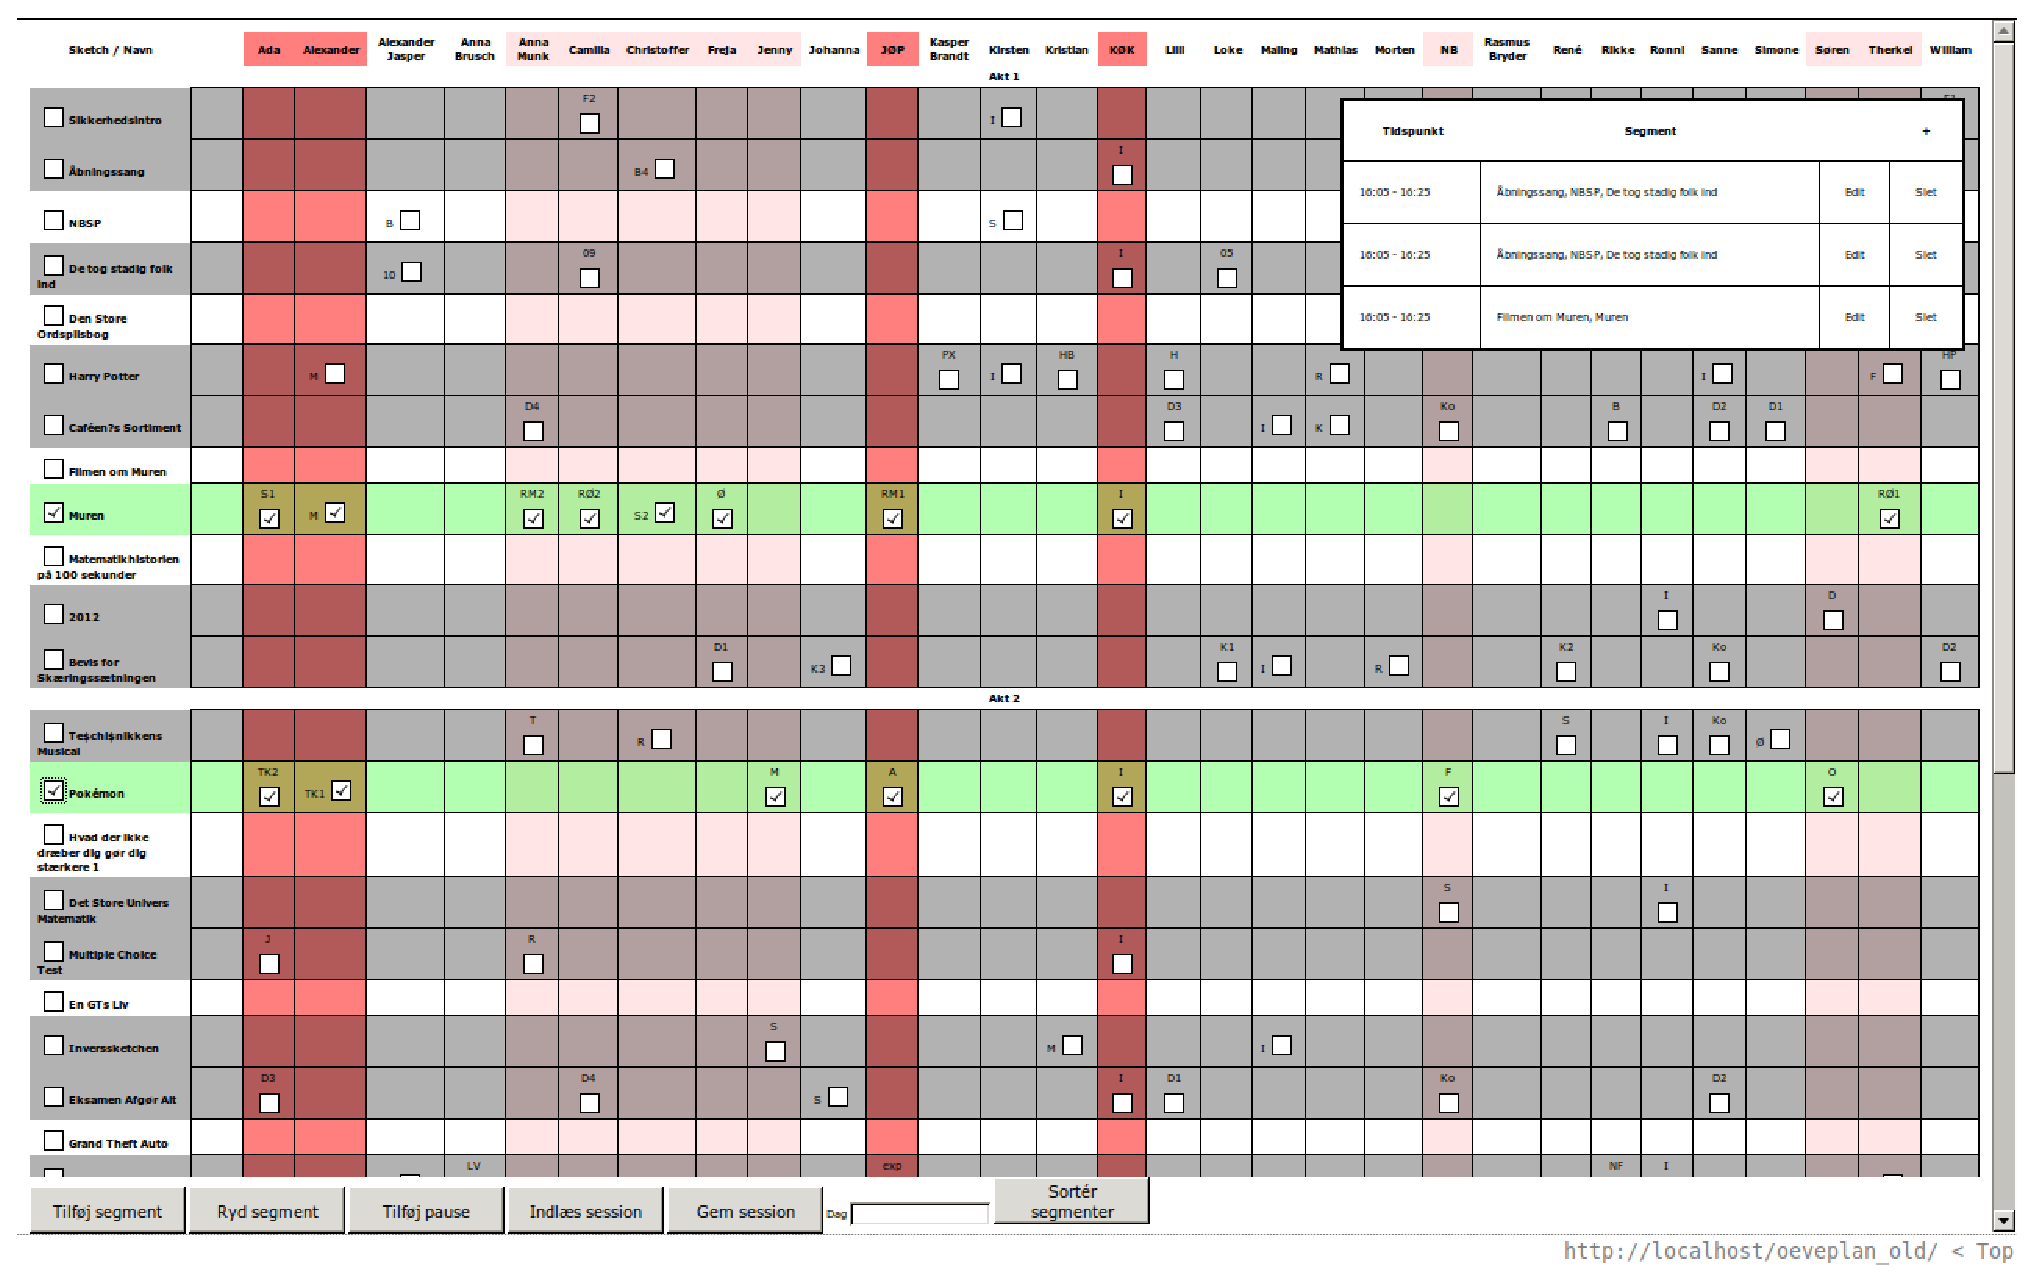
\includegraphics[width=\textwidth]{oveplan-example}
\end{center}
\end{figure}
\subsection{Installation og konfiguration}
Øveplanlægningsscriptet kan findes på
\url{http://github.com/dikurevy/oeveplan}. Scriptet er stadig under
kraftig udvikling der har indflydelse på installation og konfiguration
af scriptet. Når dette er stabilt vil der komme yderligere dokumentation. Indtil da
kontakt mig på \texttt{ronni@diku.dk} for installationsvejledning.
\subsection{Brug af øveplanlægningsscriptet}
\section{Mikrofonplan}
Mikronfplanlægningsscriptet gør det muligt at lave en mikrofonplan
udelukkende ved hjælp af drag 'n' drop. Det er muligt at tildele hver
enkelt mikrofon navn og farve og let fjerne folk fra en sketch som ikke
behøver have en mikrofon.  Dokumentation kommer i en
efterfølgende version af denne vejledning.
\begin{figure}[H]
\begin{center}
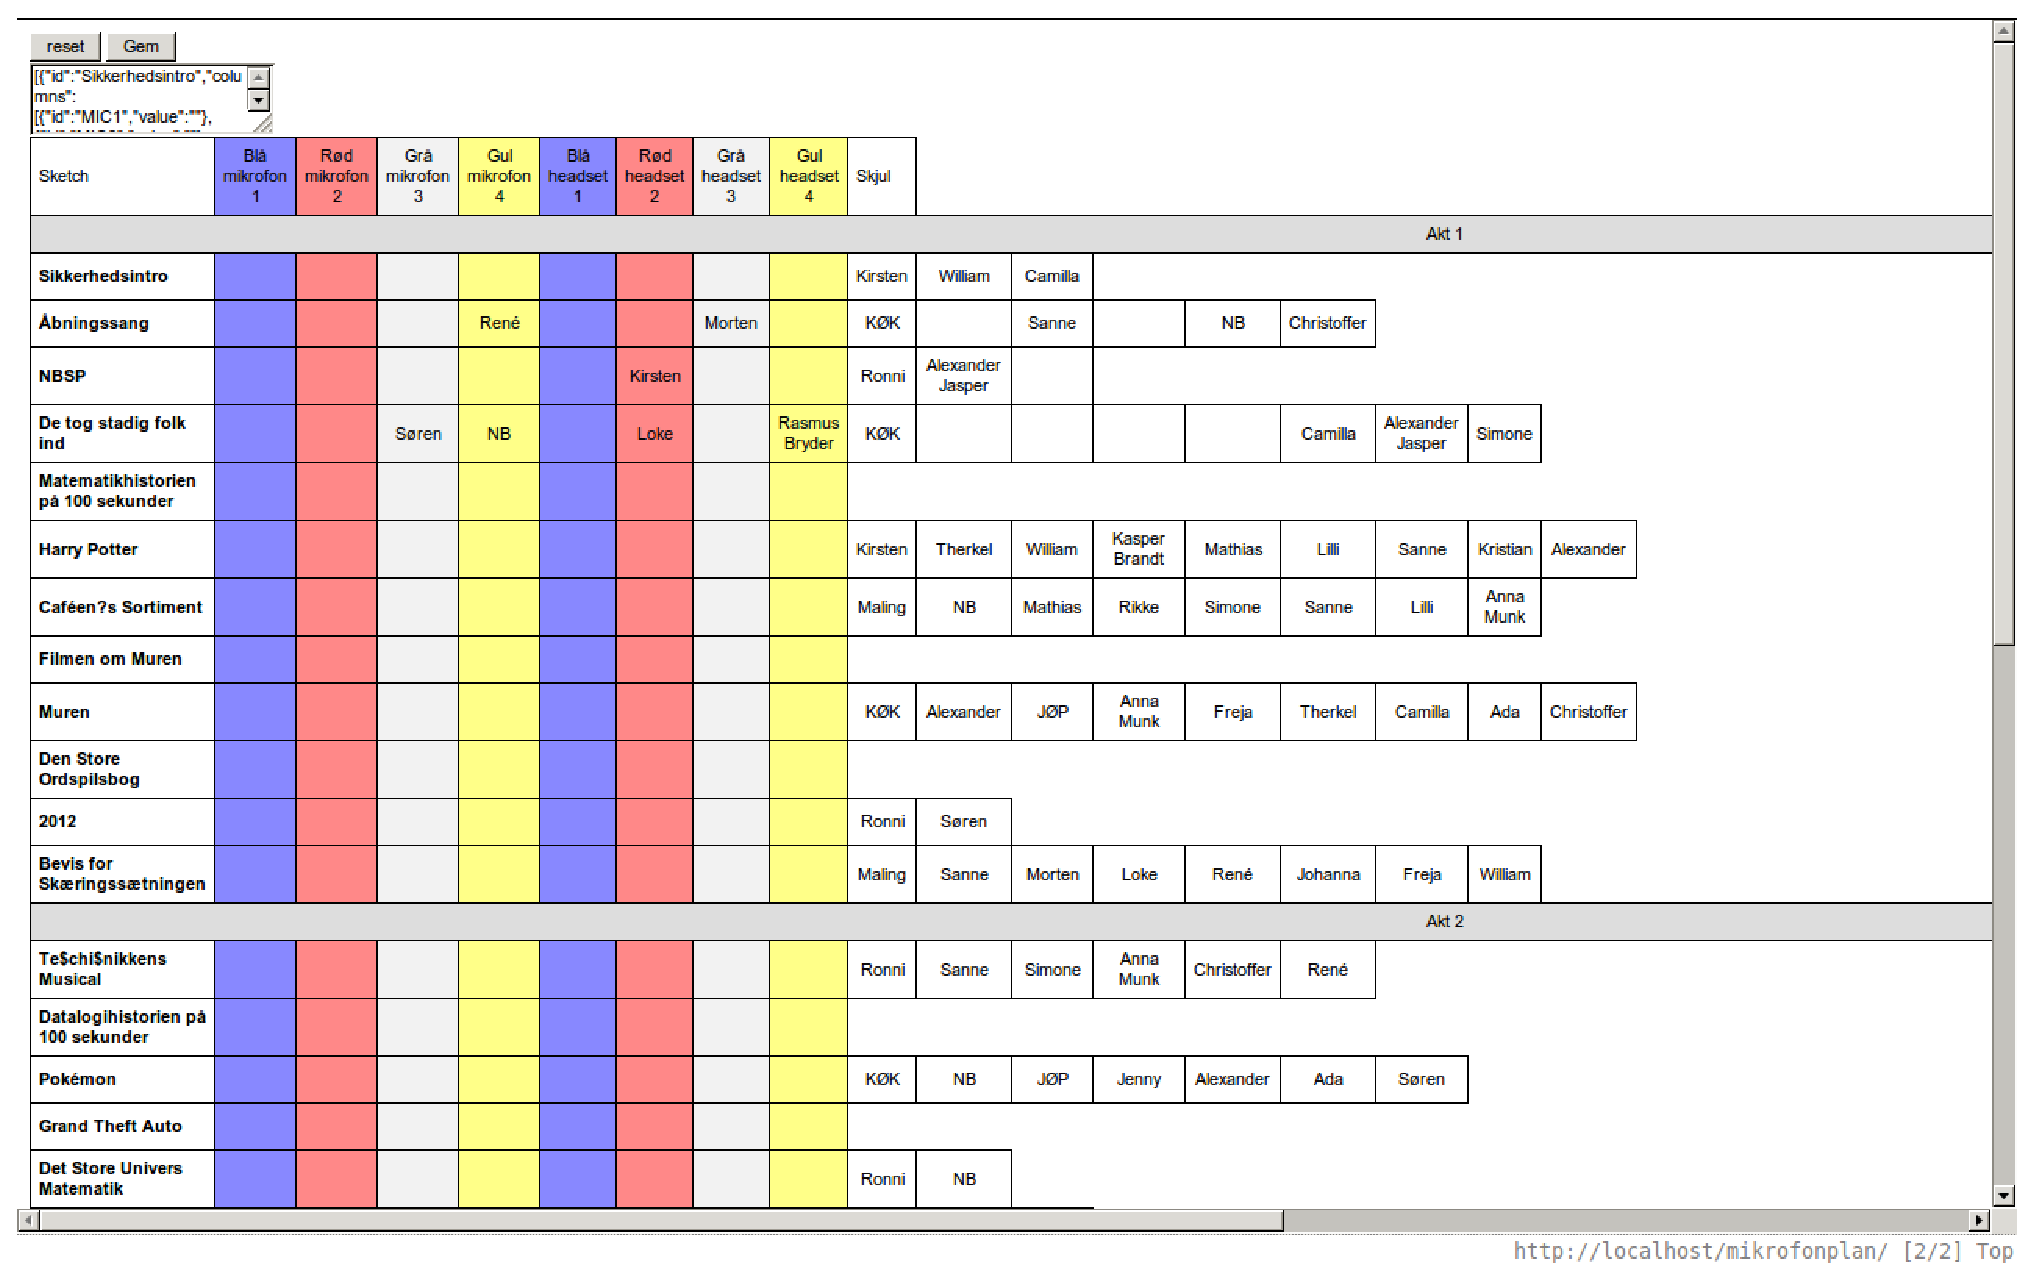
\includegraphics[width=\textwidth]{mikrofonplan-example}
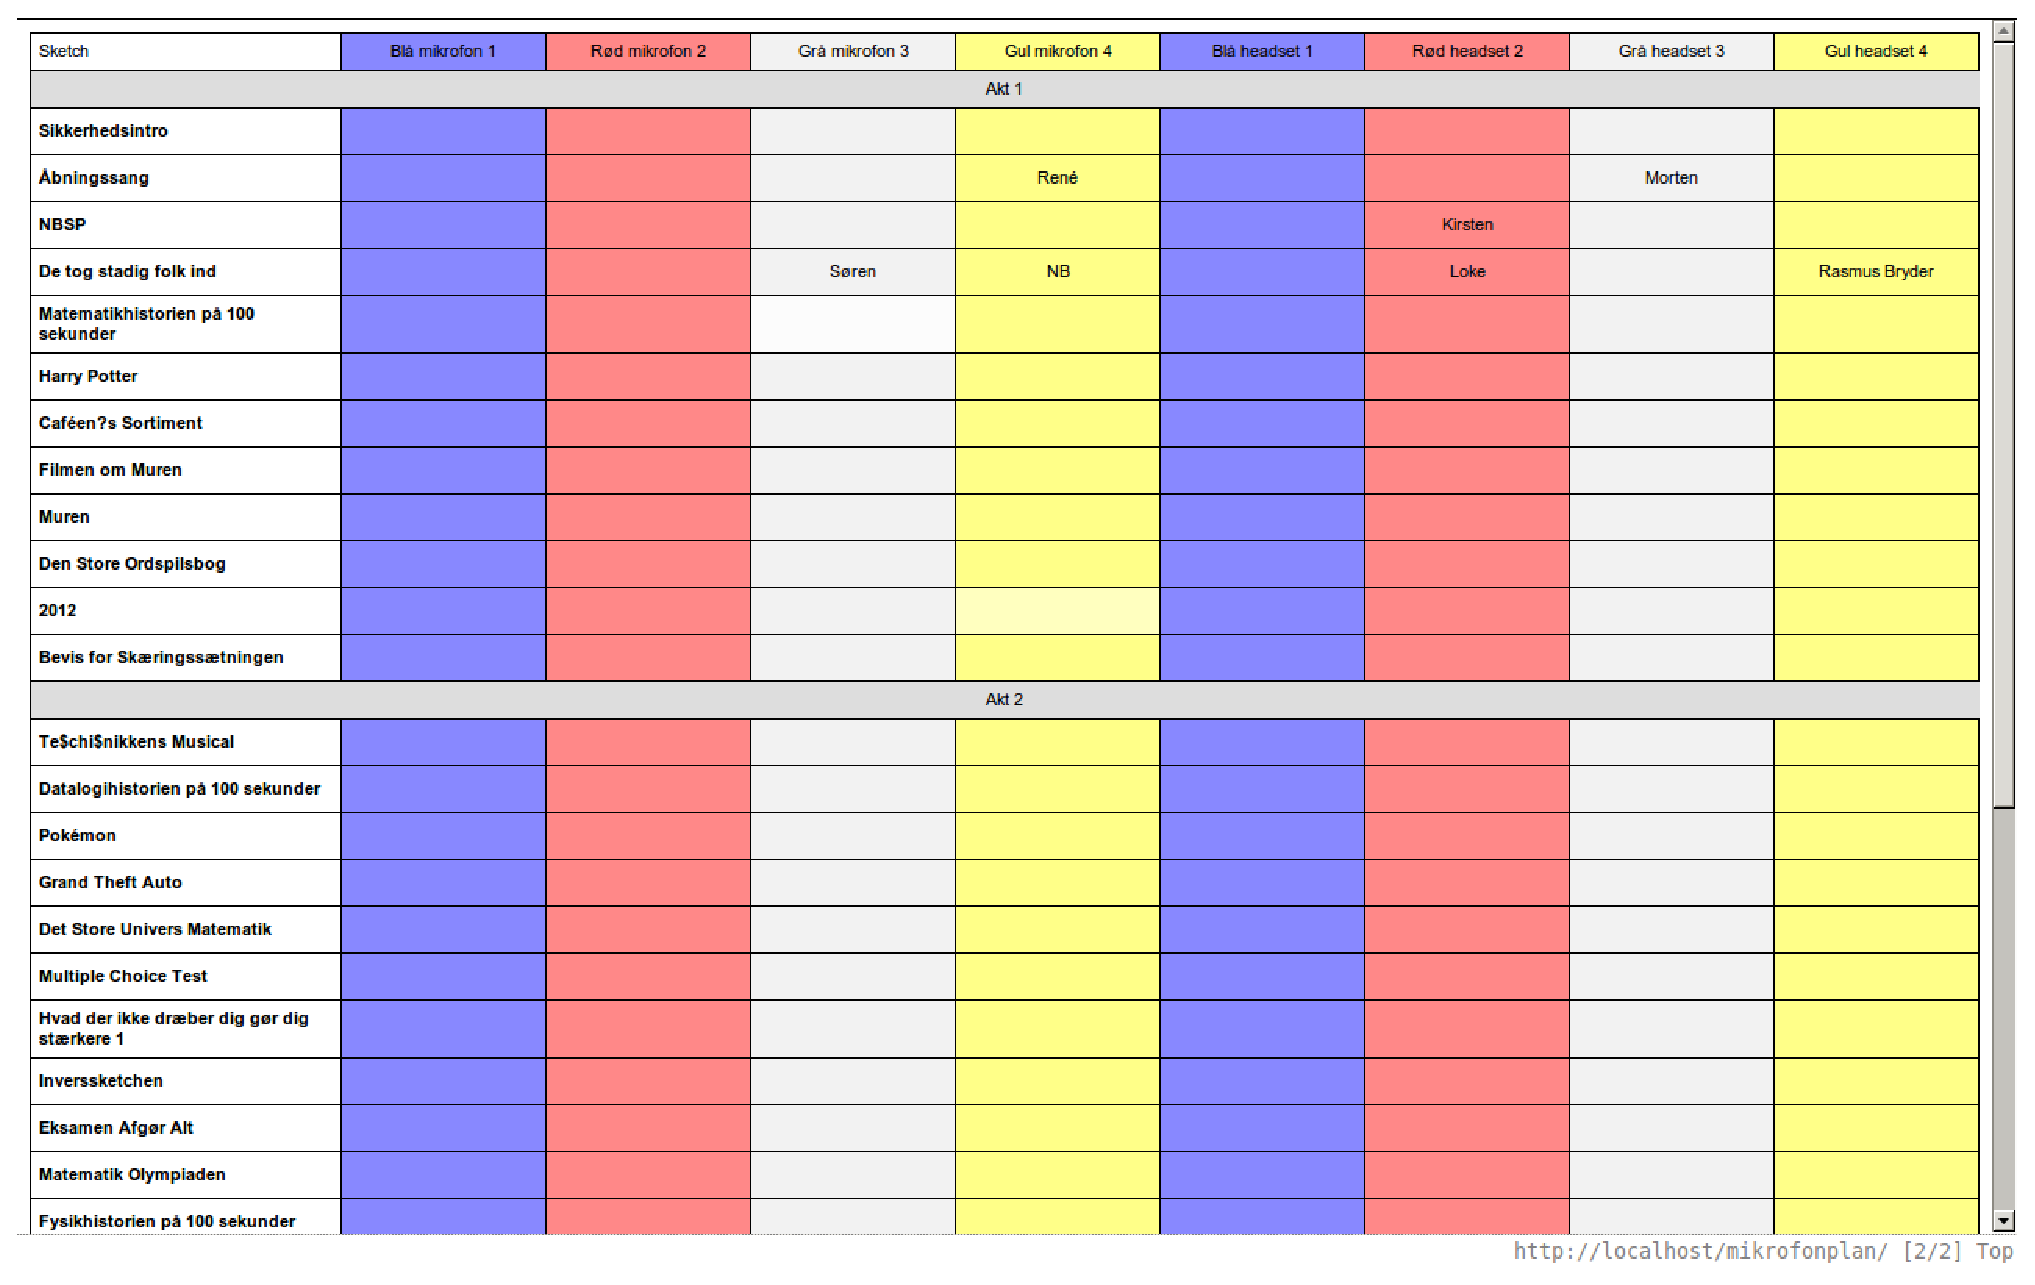
\includegraphics[width=\textwidth]{mikrofonplan-example2}
\end{center}
\end{figure}
\subsection{Installation og konfiguration}
Mikrofonplanlægningsscriptet kan findes på
\url{http://github.com/dikurevy/mikrofonplan}. Scriptet er stadig under
kraftig udvikling der har indflydelse på installation og konfiguration
af scriptet. Når dette er stabilt vil der komme yderligere dokumentation. Indtil da
kontakt mig på \texttt{ronni@diku.dk} for installationsvejledning.
\subsection{Brug af mikrofonplanlægningsscriptet}
\end{document}

